% Options for packages loaded elsewhere
\PassOptionsToPackage{unicode}{hyperref}
\PassOptionsToPackage{hyphens}{url}
%
\documentclass[
]{article}
\usepackage{lmodern}
\usepackage{amssymb,amsmath}
\usepackage{ifxetex,ifluatex}
\ifnum 0\ifxetex 1\fi\ifluatex 1\fi=0 % if pdftex
  \usepackage[T1]{fontenc}
  \usepackage[utf8]{inputenc}
  \usepackage{textcomp} % provide euro and other symbols
\else % if luatex or xetex
  \usepackage{unicode-math}
  \defaultfontfeatures{Scale=MatchLowercase}
  \defaultfontfeatures[\rmfamily]{Ligatures=TeX,Scale=1}
\fi
% Use upquote if available, for straight quotes in verbatim environments
\IfFileExists{upquote.sty}{\usepackage{upquote}}{}
\IfFileExists{microtype.sty}{% use microtype if available
  \usepackage[]{microtype}
  \UseMicrotypeSet[protrusion]{basicmath} % disable protrusion for tt fonts
}{}
\makeatletter
\@ifundefined{KOMAClassName}{% if non-KOMA class
  \IfFileExists{parskip.sty}{%
    \usepackage{parskip}
  }{% else
    \setlength{\parindent}{0pt}
    \setlength{\parskip}{6pt plus 2pt minus 1pt}}
}{% if KOMA class
  \KOMAoptions{parskip=half}}
\makeatother
\usepackage{xcolor}
\IfFileExists{xurl.sty}{\usepackage{xurl}}{} % add URL line breaks if available
\IfFileExists{bookmark.sty}{\usepackage{bookmark}}{\usepackage{hyperref}}
\hypersetup{
  pdftitle={The statistical analysis of non-linear longitudinal data in biomedical research using generalized additive models},
  pdfauthor={Ariel Mundo; Timothy J. Muldoon; John R. Tipton},
  hidelinks,
  pdfcreator={LaTeX via pandoc}}
\urlstyle{same} % disable monospaced font for URLs
\usepackage[margin=1in]{geometry}
\usepackage{longtable,booktabs}
% Correct order of tables after \paragraph or \subparagraph
\usepackage{etoolbox}
\makeatletter
\patchcmd\longtable{\par}{\if@noskipsec\mbox{}\fi\par}{}{}
\makeatother
% Allow footnotes in longtable head/foot
\IfFileExists{footnotehyper.sty}{\usepackage{footnotehyper}}{\usepackage{footnote}}
\makesavenoteenv{longtable}
\usepackage{graphicx,grffile}
\makeatletter
\def\maxwidth{\ifdim\Gin@nat@width>\linewidth\linewidth\else\Gin@nat@width\fi}
\def\maxheight{\ifdim\Gin@nat@height>\textheight\textheight\else\Gin@nat@height\fi}
\makeatother
% Scale images if necessary, so that they will not overflow the page
% margins by default, and it is still possible to overwrite the defaults
% using explicit options in \includegraphics[width, height, ...]{}
\setkeys{Gin}{width=\maxwidth,height=\maxheight,keepaspectratio}
% Set default figure placement to htbp
\makeatletter
\def\fps@figure{htbp}
\makeatother
\setlength{\emergencystretch}{3em} % prevent overfull lines
\providecommand{\tightlist}{%
  \setlength{\itemsep}{0pt}\setlength{\parskip}{0pt}}
\setcounter{secnumdepth}{5}
\usepackage{subfig}
\usepackage{breqn}

\title{\textbf{The statistical analysis of non-linear longitudinal data in biomedical research using generalized additive models}}
\usepackage{etoolbox}
\makeatletter
\providecommand{\subtitle}[1]{% add subtitle to \maketitle
  \apptocmd{\@title}{\par {\large #1 \par}}{}{}
}
\makeatother
\subtitle{\emph{Beyond repeated measures ANOVA and Linear Mixed Models}}
\author{Ariel Mundo\footnote{Department of Biomedical Engineering, University of Arkansas, Fayetteville} \and Timothy J. Muldoon\footnote{Department of Biomedical Engineering, University of Arkansas, Fayetteville} \and John R. Tipton\footnote{Department of Mathematical Sciences, University of Arkansas, Fayetteville}}
\date{}

\begin{document}
\maketitle

{
\setcounter{tocdepth}{2}
\tableofcontents
}
\hypertarget{background}{%
\section{Background}\label{background}}

A longitudinal study is defined as that which is designed to repeatedly measure a variable of interest in a group (or groups) of subjects. In biomedical research, this type of study is employed when the intention is to observe the evolution of the effect of a certain treatment across time, rather than analyzing it at a single time point (a cross-sectional study). Clinical studies of breast and neck cancer have used a longitudinal approach {[}1{]}, {[}2{]}. In the first case, weekly measurements of skin toxicities in patients with radiation-induced dermatitis were taken for up to 8 weeks; whereas in the latter mouth opening was assessed at 6,12, 18, 24 and 36 months after radiotherapy (RT). Longitudinal studies have beenn also used to analyze tumor response {[}3{]}--{[}6{]}, antibody expression {[}7{]}, {[}8{]}, and cell metabolism {[}9{]}, {[}10{]}.

Traditionally, a ``frequentist'' approach is used in biomedical research to derive inferences from a longitudinal study. Such statistical view derives its name from the fact that it regards probability as a limiting frequency{[}11{]} and its application is based on a null hypothesis test using the \emph{analysis of variance over repeated measures} (repeated measures ANOVA or rm-ANOVA). This methodology makes two key assumptions regarding longitudinal data: constant correlation exists across same-subject measurements, and observations from each subject are obtained at all time points through the study (a condition also known as complete observations) {[}12{]}, {[}13{]}.

However, constant correlation is frequently unjustified as its value tends to diminish between measures when the time interval between them increases {[}14{]}.
In the case of the number of observations during the study, different situations can arise that prevent the collection of complete measurements for all subjects: in a clinical trial voluntary withdrawal from one or multiple patients can occur, whereas attrition in animals due to injury or weight loss can occur in preclinical experiments, and it is even possible that unexpected complications with equipment or supplies arise, preventing the researcher from collecting measurements at a certain time point and therefore violating the \emph{complete observations} assumption of rm-ANOVA.

When incomplete observations occur, an rm-ANOVA requires the exclusion of all subjects with missing observations from the analysis. This can result in increased costs if the desired statistical power is not met with the remaining observations, as it would be necessary to enroll more subjects. At the same time, if the excluded observations contain insightful information that is not used, their elimination from the analysis may limit the demonstration of significant differences between groups. Additionally, rm-ANOVA uses a \emph{post hoc} analysis to assess differences between the measured response in different groups. A \emph{post hoc} analysis is based on multiple repeated comparisons to estimate a \emph{p-value}, a metric that is widely used as a measure of significance. Because the \emph{p-value} is highly variable, multiple comparisons can inflate the false positivity rate {[}15{]}, {[}16{]}, consequently biasing the conclusions of the study.

During the last decade, the biomedical community has started to recognize the limitations of rm-ANOVA in the analysis of longitudinal information. This is exemplified by the use of linear mixed effects models (LMEMs) in certain groups to analyze longitudinal data {[}10{]}, {[}17{]}. Briefly, these models incorporate \emph{fixed effects}, which correspond to the levels of experimental factors in the study (e.g.~the different drug regimens in a clinical trial), and \emph{random effects}, which account for random variation within the population. These models are more flexible than the traditional rm-ANOVA as they can accommodate missing observations for multiple subjects and allow different modeling strategies for the variability within each measure in every subject {[}18{]}. On the other hand, they impose restrictions in the distribution of the errors of the random effects {[}12{]}.

One final assumption that is not initially evident for both rm-ANOVA and LMEMs models pertains the relationship between the observed effect and the progression of the timeline of the study, which is expected to be linear {[}18{]}. This common assumption in both rm-ANOVA ane LMEMs consequently restricts the inferences from the model when the data does not follow a linear trend. In biomedical research, a special case of this behavior in longitudinal data arises in measurements of tumor response in preclinical and clinical settings {[}3{]}, {[}10{]}, {[}17{]}. These studies have shown that the collected signal does not follow a linear trend over time, and presents extreme variability at different time points, making the fit of and the estimations of an LMEM or rm-ANOVA model inconsistent with the observed variation. In other words, the in both cases the model tries to explain highly-variable data using a linear trend, consequently biasing the estimates. Additionally, although it is possible that a \emph{post hoc} analysis is able to find ``significant'' \emph{p-values}( \emph{p}\textless0.05) by using multiple comparisons between the model terms, the use of this estimator is limited in such scenario because it is intended to work in models that have a reasonable agreement with the data.

As the ``frequentist'' rm-ANOVA and the more advanced LMEM approach are both limited in the analysis of non-linear longitudinal information, there is a need for biomedical researchers to explore the use of additional statistical tools that allow the information (and not an assumed trend) to determine the fit of the model, while enabling inferences that are both adequate and consistent from a statistical perspective.
In this regard, Generalized Additive Models (GAMs) present an alternative approach to analyze longitudinal data. Although not commonly used in the biomedical community, these non-parametric models have been used to analyze temporal variations in geochemical and palaeoecological data {[}19{]}--{[}21{]}, health-environment interactions {[}22{]} and political science {[}23{]} . There are several advantages of GAMs over LMEMs and rm-ANOVA models: They have an extensively developed theoretical background, enable the data to dictate the trend of the model, can accommodate missing observations and do not require constant correlation between repeated measurements {[}24{]}.Therefore, GAMs can provide a more suitable statistical method to analyze non-linear biomedical longitudinal data.

The current advances in programming languages designed for statistical analysis (specifically \(\textsf{R}\)), have eased the computational implementation of more complex models beyond LMEMs. In particular, \(\textsf{R}\) has an extensive collection of documentation and functions to fit GAMs in the package \emph{mgcv} {[}24{]}--{[}26{]} that not only speed up the initial stages of the analysis but enable the use of advanced modeling structures (e.g.~hierarchical models, confidence interval comparisons) without requiring advanced programming skills from the user. This programming language is also able to simulate data, an emerging strategy used to test statistical models {[}27{]}. This allows to create and explore different alternatives for analysis without collecting information in the field, and reduces the time window between experiment design and its implementation.

Therefore, the purpose of this study is to provide biomedical researchers with a clear understanding of the theory and the practical implementation of GAMs to analyze longitudinal data using by focusing on four areas. First, the limitations of rm-ANOVA and LMEMs to analyze longitudinal data are contrasted in the cases of missing observations, assumption of linearity and correlation structures. Secondly, the key theoretical elements of GAMS are presented without using extensive derivations or complex mathematical notation that can obscure their understanding. Thirdly, simulated data that follows the trend of previously reported values {[}17{]} is used to illustrate the type of non-linear longitudinal data that occurs in biomedical research and the implementation of GAMs in such scenario. Finally, reproducibility is emphasized by providing the code to generate the data and the implementation of GAMs in \(\textsf{R}\), in conjunction with a step-by-step guide to fit models of increasing complexity.\\
In summary, the exploration of modern statistical techniques to analyze longitudinal data may allow biomedical researchers to consider the use of GAMs instead of rm-ANOVA or LMEMs when the data does not follow a linear trend, and will also help to improve the standards for reproducibility in biomedical research.

\hypertarget{challenges-presented-by-longitudinal-studies}{%
\section{Challenges presented by longitudinal studies}\label{challenges-presented-by-longitudinal-studies}}

\hypertarget{the-frequentist-case-for-longitudinal-data}{%
\subsection{The ``frequentist'' case for longitudinal data}\label{the-frequentist-case-for-longitudinal-data}}

The \emph{repeated measures analysis of variance} (rm-ANOVA) is the standard statistical analysis for longitudinal data in biomedical research, but certain assumptions are necessary to make the model valid. From a practical view, they can be divided in three areas: linear relationship between covariates and response, constant correlation between measurements, and complete observations for all subjects. Each one of these assumptions is discussed below.

\hypertarget{linear-relationship}{%
\subsection{Linear relationship}\label{linear-relationship}}

In a biomedical longitudinal study, two or more groups of subjects (patients, mice, samples) are subject to a different treatments (e.g.~a ``treatment'' group receives a novel drug vs.~a ``control'' group that receives a placebo), and measurements from each subject within each group are collected at specific time points. The collected response has both \emph{fixed} and \emph{random} components. The \emph{fixed} component can be understood as a constant value in the response which the researcher is interested in measuring, i.e, the effect of the novel drug in the ``treatment'' group.The \emph{random} component can be defined as ``noise'' caused by some inherent variability within the study. For example, if the blood concentration of the drug is measured in certain subjects in the early hours of the morning while others are measured in the afternoon, it is possible that the difference in the collection time of the measurement introduces some ``noise'' in the signal. As their name suggests, this ``random'' variability needs to be modeled as a variable rather than as a constant value.

Mathematically speaking, a rm-ANOVA model can be written as:

\begin{equation}
y_{i} = \mu+ \beta_1* time_{t} + \beta_2* treatment_{j} + \beta_3* time_{t}*treatment_{j}+\pi_{ij} +\epsilon_{tij}\\ 
\label{eq:linear-model}
\end{equation}

In this model \(y_i\) is the response by subject \(i\), which can be decomposed in a mean value \(\mu\), \emph{fixed effects} of time (\(time_t\)), treatment (\(time_j\)) and their interaction; a \emph{random effect} \(\pi_{ij}\) of each subject within each group, and errors per subject per time per group \(\epsilon_{tij}\).
Suppose two treatments groups are used in the study. Models per group can be generated if 0 is used for the first treatment group (Group A) and 1 for the second treatment group (Group B). The linear models then become:

\begin{equation}
y = \begin{cases}
\mu + \beta_1*time_{t}+\epsilon_{ti}   & \mbox{if Group A}\\
\mu + \beta_1 * time_{t} + \beta_2 * treatment_{j} +\beta_3* time_{t} * treatment_{j}+\pi_{i}+\epsilon_{tij}  & \mbox{if Group B}\\
\end{cases}
\label{eq:ANOVA-by-group}
\end{equation}

Furthermore, \eqref{eq:ANOVA-by-group} can be re-written under the generalized linear model (GLM) framework {[}28{]}. The main difference in this case is that a GLM model uses a \emph{linking function} to connect the observed value to the linear model.

Thus,

\begin{equation}
  y =\mu +\boldsymbol{\beta}_1* f(time) + \beta_2* treatment+ \\
  \boldsymbol{\beta}_3* f(time)*treatment \\
  \label{eq:GLM}
  \end{equation}

The linear model in \eqref{eq:linear-model} is a GLM where \(f(time) = time\) with the identity function \(f(x) = x\). If the GLM is then written in terms of two treatment groups as in \eqref{eq:ANOVA-by-group}, the model becomes:

\begin{equation}
  y = \begin{cases}
  \mu +\boldsymbol{\beta}_1* f(time)  & \mbox{if Group A} \\
  \mu +\boldsymbol{\beta}_1* f(time)  + \beta_2* treatment + \boldsymbol{\beta}_3* f(time) *treatment   
  & \mbox{if Group B}\\
  \end{cases}
  \label{eq:GLM-by-group}
\end{equation}

Regardless of its presentation, \eqref{eq:linear-model}, \eqref{eq:ANOVA-by-group} and \eqref{eq:GLM-by-group} show that the model expects a linear relationship between the covariates and the response. When the data does not follow a linear trend, the fit that the model produces does not accurately represent the changes in the data. To exemplify this consider simulated longitudinal data where the a normally distributed response of two groups of 10 subjects each is obtained, and an rm-ANOVA model identical to \eqref{eq:linear-model} is fitted to the data using the package \emph{nlme} (the code for the simulated data and models is available in the Appendix).

\begin{figure}
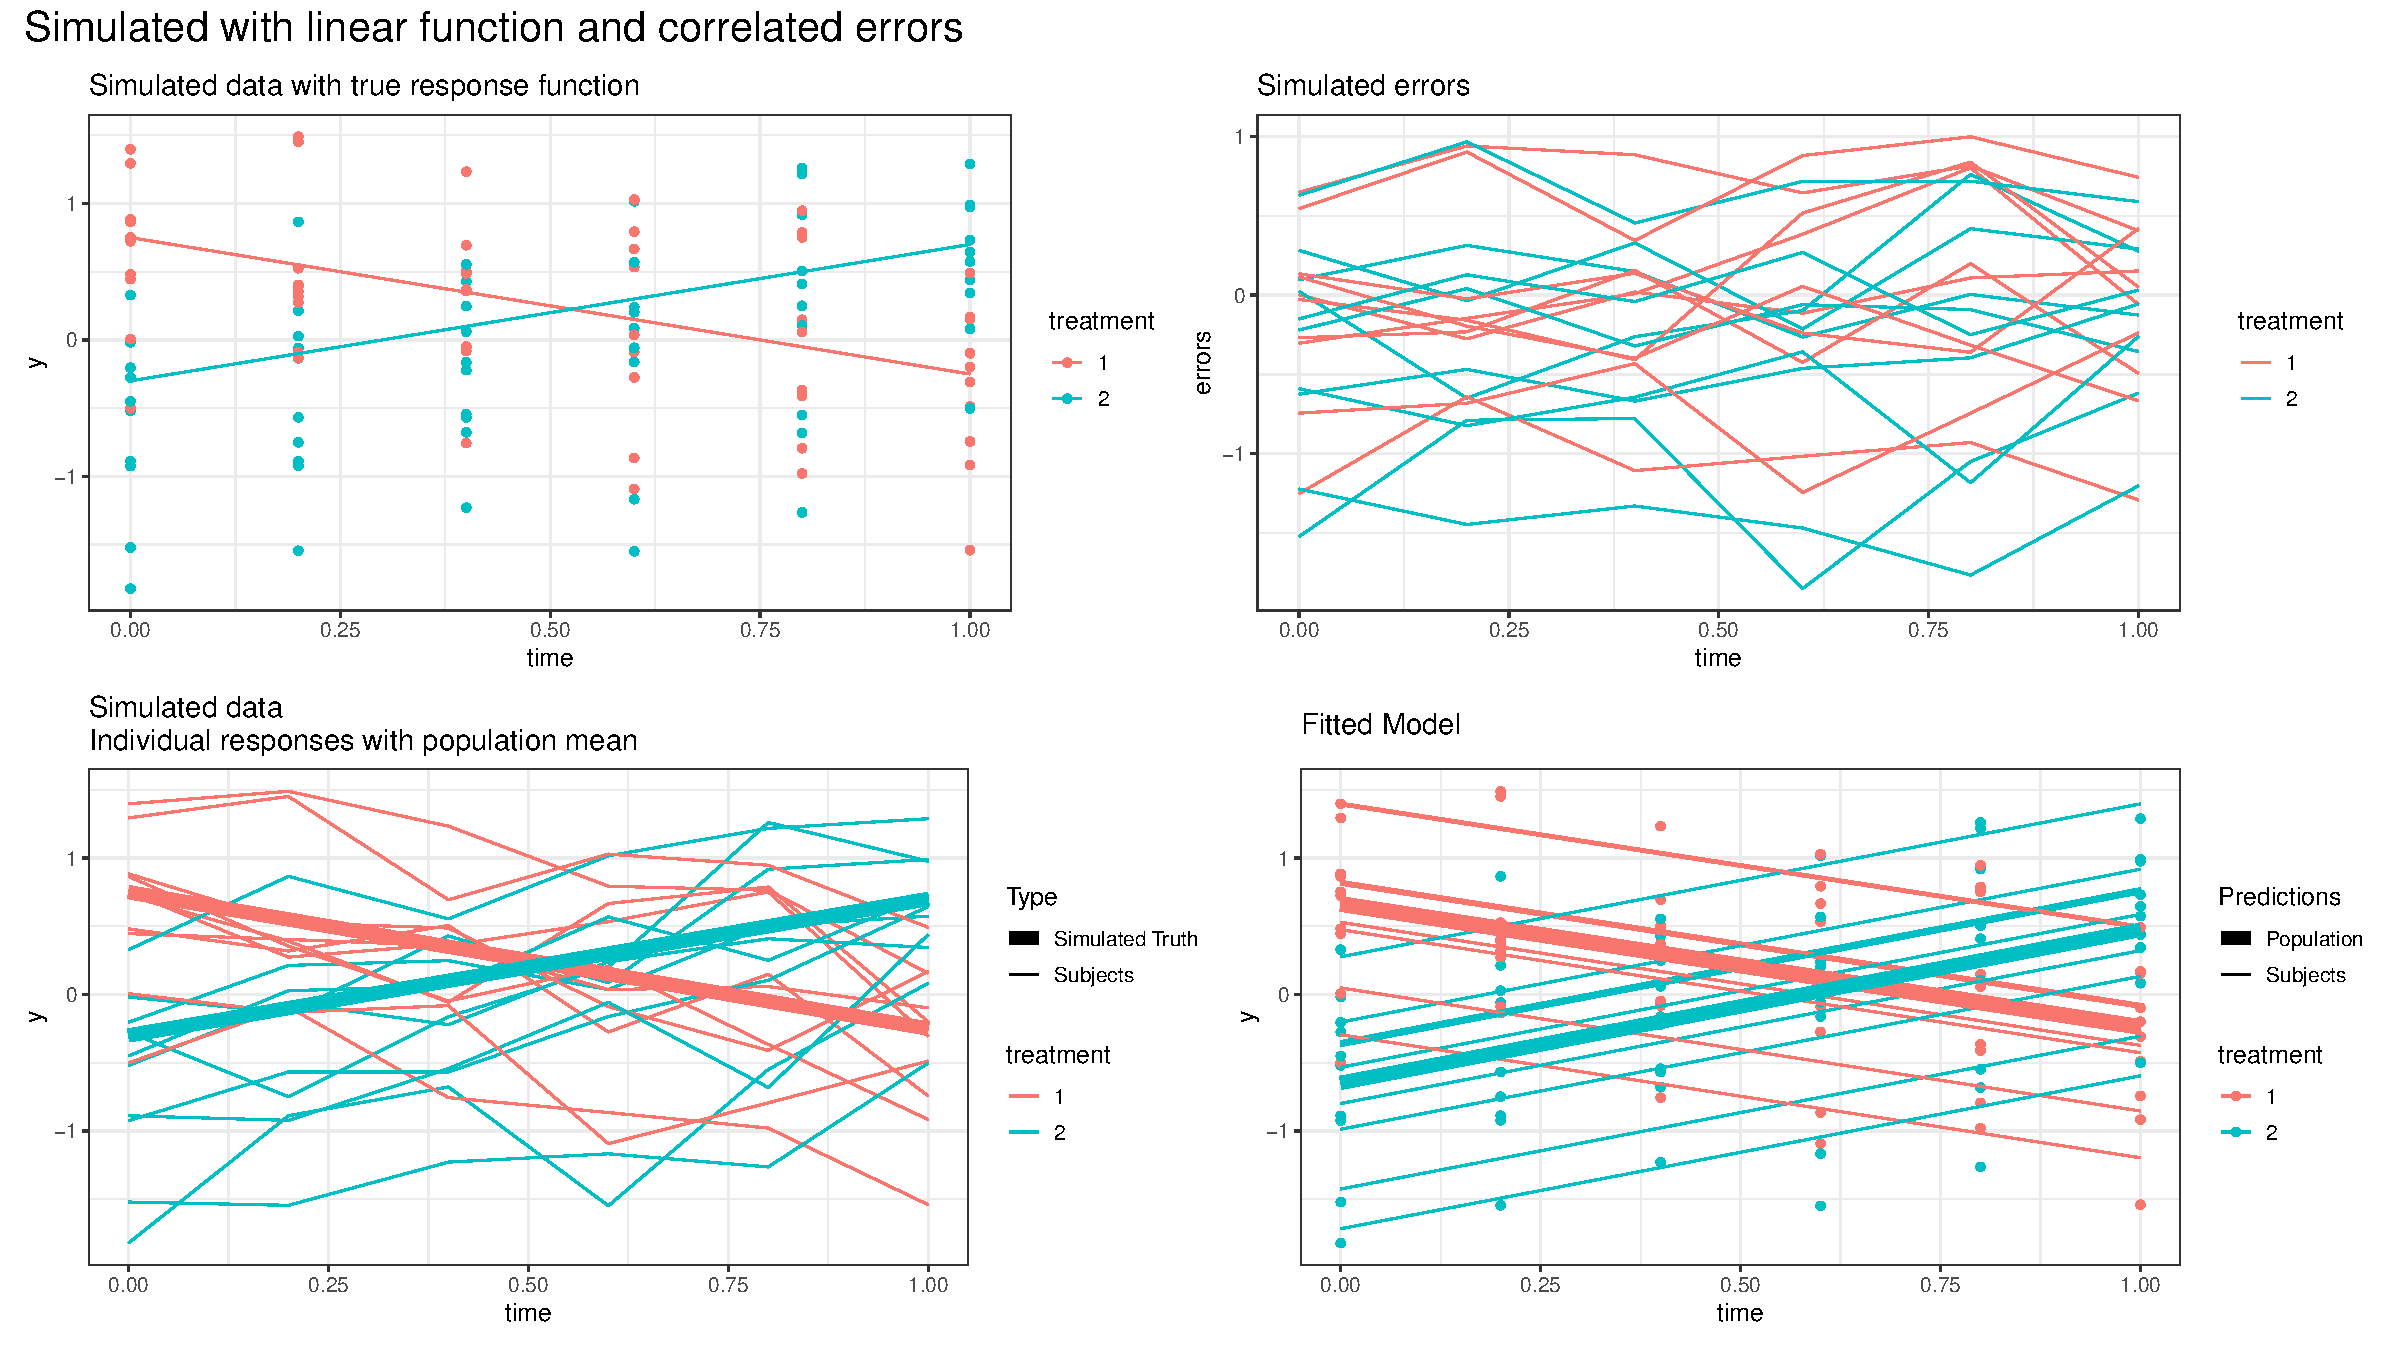
\includegraphics[width=1\linewidth]{Manuscript_AM_v1_files/figure-latex/linear-model-1} \caption{Simulated linear responses from two groups with a rm-ANOVA model fitted. Top row, simulated data, lines represent mean response. Bottom row, fitted model, thick lines represent predicted mean response }\label{fig:linear-model}
\end{figure}

It is clear from \ref{fig:linear-model} that the fit produced by the rm-ANOVA model is good as the predictions for the mean response are identical to the ``truth'' of the simulated data.

However, consider the case when the data follows a non-linear trend, such as the one simulated in \ref{fig:quadratic-response}. Here, the simulated data follows a quadratic behavior. It is clear from the figure that changes in each group occur through the timeline, although the final mean value is the same as the initial value. Fitting an rm-ANOVA model like \eqref{eq:linear-model} again produces the fit that appears at the bottom of \ref{fig:quadratic-response}.

\begin{figure}
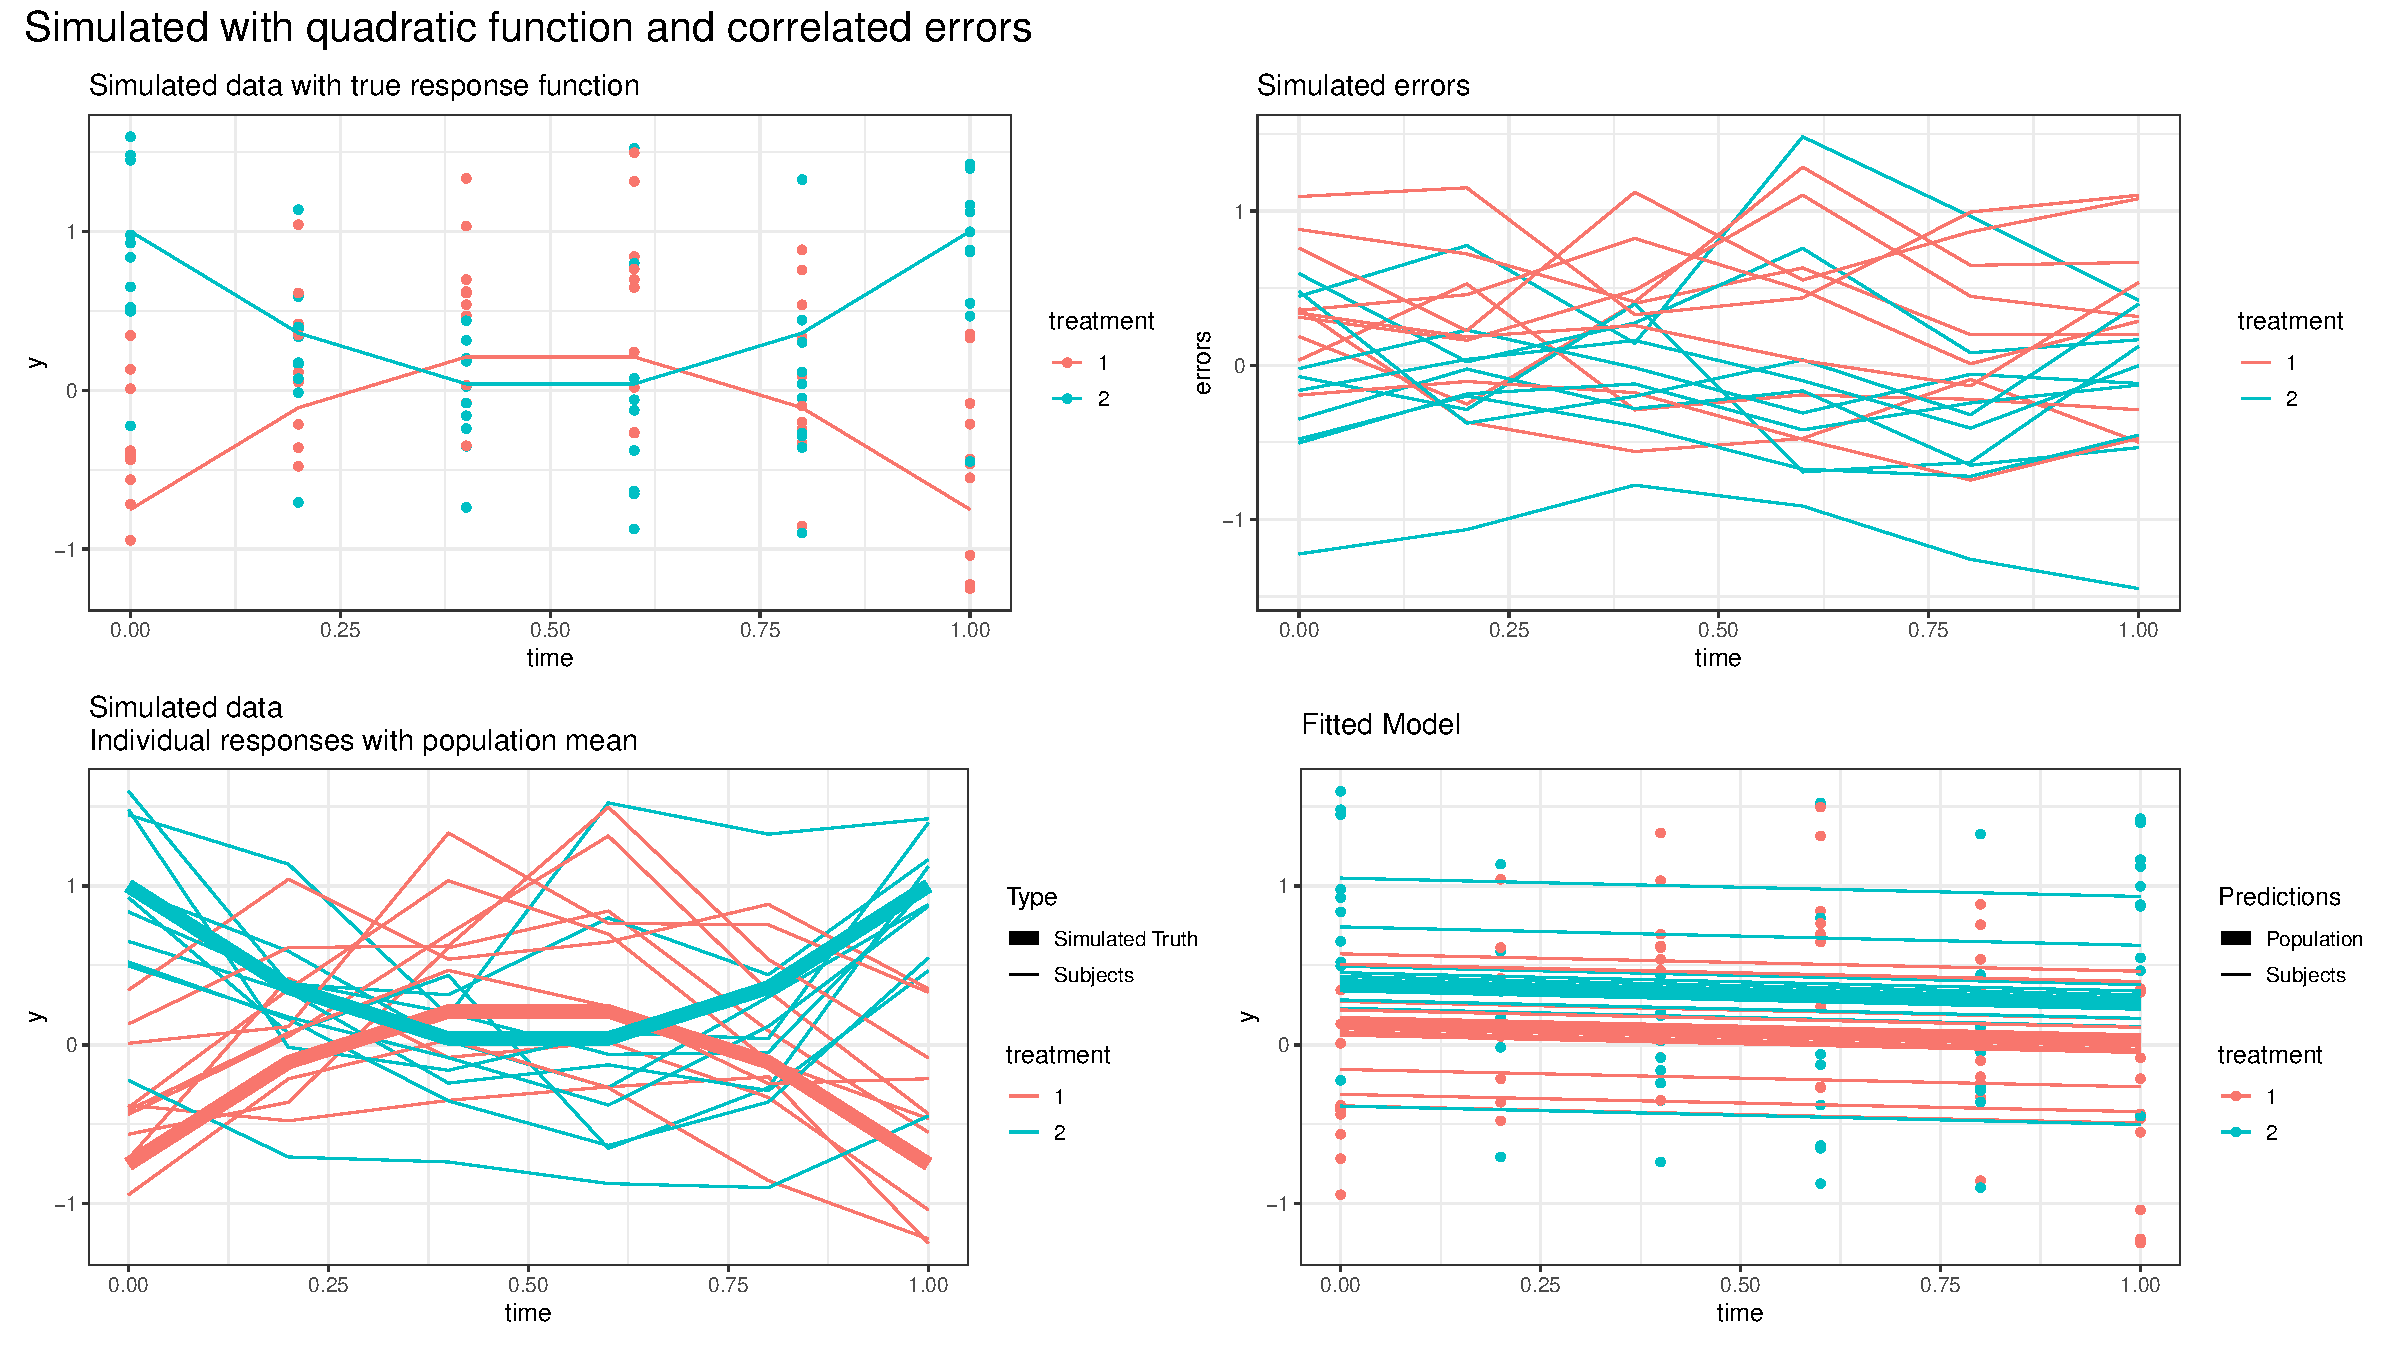
\includegraphics[width=1\linewidth]{Manuscript_AM_v1_files/figure-latex/quadratic-response-1} \caption{Simulated quadratic responses from two groups with an rm-ANOVA model fitted. Top row, simulated data, lines represent mean response. Bottom row, fitted model, thick lines represent predicted mean response}\label{fig:quadratic-response}
\end{figure}

In this case, when the predictions are compared to the simulated data it is clear that the model is not capturing the changes within each group throughout the timeline. This highlights the limitation of rm-ANOVA and LMEMs with longitudinal non-linear data, where the variations are not captured and modeled properly.

\hypertarget{covariance-in-rm-anova-and-lmems}{%
\subsection{Covariance in rm-ANOVA and LMEMs}\label{covariance-in-rm-anova-and-lmems}}

In a longitudinal study there is an expected \emph{variance} between repeated measurements on the same subject, and because repeated measures occur in the subjects within each group, there is a \emph{covariance} between measurements at each time point within each group. The \emph{covariance matrix} (also known as the variance-covariance matrix) is a matrix that captures the variation between and within subjects in a longitudinal study{[}29{]} (For an in-depth analysis of the covariance matrix see {[}30{]}, {[}31{]}).

In the case of an rm-ANOVA analysis, it is assumed that the covariance matrix has a specific construction known as \emph{compound symmetry} (also known as ``sphericity'' or ``circularity''). Under this assumption, the between-subject variance and within-subject correlation are constant across time {[}31{]}--{[}33{]}. However, it has been shown that this condition is frequently unjustified because the correlation between measurements tends to change over time {[}34{]}; and it is higher between consecutive measurements {[}12{]}, {[}14{]}. Although corrections can be made (such as Huyhn-Feldt or Greenhouse-Geisser) the effectiveness of each correction is limited because it depends on the size of the sample,the number of repeated measurements{[}27{]}, and they are not robust if the group sizes are unbalanced {[}35{]}. In other words, if the data does not present constant correlation between repeated measurements, the assumptions required for an rm-ANOVA model are not met and the use of corrections may still not provide a reasonable adjustment that makes the model valid.

In the case of LMEMs, one key advantage over rm-ANOVA is that they allow different structures for the variance-covariance matrix including exponential, autoregressive of order 1, rational quadratic and others {[}18{]}. Nevertheless, the analysis required to determine an appropriate variance-covariance structure for the data can be a long process by itself. Overall, the spherical assumption for rm-ANOVA may not capture the natural variations of the correlation in the data, and can bias the inferences from the analysis.

\hypertarget{missing-observations}{%
\subsection{Missing observations}\label{missing-observations}}

Missing observations are an issue that arises frequently in longitudinal studies. In biomedical research, this situation can be caused by reasons beyond the control of the investigator {[}molenberghs2004{]}.Dropout from patients, or attrition or injury in animals are among the reasons for missing observations. Statistically, missing information can be classified as \emph{missing at random} (MAR), \emph{missing completely at random} (MCAR), and \emph{missing not at random} (MNAR) {[}31{]}. In a MAR scenario, the pattern of the missing information is related to some variable in the data, but it is not related to the variable of interest {[}36{]}. If the data are MCAR, this means that the missigness is completely unrelated to the collected information {[}37{]}, and in the case of MNAR the missing values are dependent on their value. An rm-ANOVA model assumes complete observations for all subjects, and therefore subjects with one or more missing observations are excluded from the analysis. This is inconvenient because the remaining subjects might not accurately represent the population, and statistical power is affected by this reduction in sample size {[}38{]}.

In the case of LMEMs, inferences from the model are valid when missing observations in the data exist that are MAR {[}30{]}. The pattern of missing observations can be considered MAR if the missing observations are not related any of the other variables measured in the study {[}34{]}. For example, if attrition occurs in all mice that had lower weights at the beginning of a chemotherapy response study, the missing data can be considered MAR because the missigness is unrelated to other variables of interest.

This section has presented the assumptions of rm-ANOVA to analyze longitudinal information and its differences when compared to LMEMs regarding to missing data and the modeling of the covariance matrix. Of notice, LMEMs offer a more robust and flexible approach than rm-ANOVA and if the data follows a linear trend, they provide an excellent choice to derive inferences from a repeated measures study. However, when the data presents high variability, LMEMs fail to capture the non-linear trend of the data. To analyze such type of data, we present generalized additive models (GAMs) as an alternative in the following section.

\hypertarget{gams-as-a-special-case-of-generalized-linear-models}{%
\section{GAMs as a special case of Generalized Linear Models}\label{gams-as-a-special-case-of-generalized-linear-models}}

A GAM is a special case of the Generalized Linear Model (GLM), a framework that allows for response distributions that do not follow a normal distribution {[}24{]}, {[}39{]}. Following the notation by Simpson {[}21{]} A GAM model can be represented as:

\begin{equation}
  y_{t}=\beta_0+f(x_t)+\epsilon_t  
  \label{eq:GAM}
\end{equation}

Where \(y_t\) is the response at time \(t\), \(\beta_0\) is the expected value at time 0, the change of \(y\) over time is represented by the function \(f(x_t)\) and \(\epsilon_t\) represents the residuals.

In contrast to rm-ANOVA or LMEMs, GAMs use \emph{smooth functions} to model the relationship between the covariates and the response. This approach is more advantageous as it does not restrict the model to a linear relationship. One possible function for \(f(x_t)\) is a polynomial, but a major limitation is that they create a ``global'' fit as they assume that the same relationship exists everywhere, which can cause problems with the fit {[}23{]}.

To overcome this limitation, the smooth functions in GAMs are represented using \emph{basis functions} over evenly spaced ranges of the covariates known as \emph{knots}. The \emph{basis function} used is a cubic spline, which is a smooth curve constructed from cubic polynomials joined together{[}21{]}, {[}24{]}. Cubic splines have a long history in their use to solve non-parametric statistical problems and are the default choice to fit GAMs as they are the simplest option to obtain visual smoothness {[}40{]}. Therefore, GAMs overcome the limitation that occurs in LMEMs and rm-ANOVA when the data is non linear, such as \ref{fig:quadratic-response}. Regarding longitudinal data, Pedersen et al {[}20{]} demonstrated the capabilities of GAMs in this area using ecological data.

The use of GAMs to analyze biomedical longitudinal data, and the impact of missing observations in the fit of the model will be examined in detail in the following section using simulation.

\begin{center}\rule{0.5\linewidth}{0.5pt}\end{center}

\hypertarget{references}{%
\section*{References}\label{references}}
\addcontentsline{toc}{section}{References}

\hypertarget{refs}{}
\leavevmode\hypertarget{ref-sio2016}{}%
{[}1{]} T. T. Sio \emph{et al.}, ``Repeated measures analyses of dermatitis symptom evolution in breast cancer patients receiving radiotherapy in a phase 3 randomized trial of mometasone furoate vs placebo (n06c4 {[}alliance{]}),'' \emph{Supportive Care in Cancer}, vol. 24, no. 9, pp. 3847--3855, 2016.

\leavevmode\hypertarget{ref-kamstra2015}{}%
{[}2{]} J. Kamstra, P. Dijkstra, M. Van Leeuwen, J. Roodenburg, and J. Langendijk, ``Mouth opening in patients irradiated for head and neck cancer: A prospective repeated measures study,'' \emph{Oral Oncology}, vol. 51, no. 5, pp. 548--555, 2015.

\leavevmode\hypertarget{ref-roblyer2011}{}%
{[}3{]} D. Roblyer \emph{et al.}, ``Optical imaging of breast cancer oxyhemoglobin flare correlates with neoadjuvant chemotherapy response one day after starting treatment,'' \emph{Proceedings of the National Academy of Sciences}, vol. 108, no. 35, pp. 14626--14631, 2011.

\leavevmode\hypertarget{ref-tank2020}{}%
{[}4{]} A. Tank \emph{et al.}, ``Diffuse optical spectroscopic imaging reveals distinct early breast tumor hemodynamic responses to metronomic and maximum tolerated dose regimens,'' \emph{Breast cancer research}, vol. 22, no. 1, pp. 1--10, 2020.

\leavevmode\hypertarget{ref-pavlov2018}{}%
{[}5{]} M. V. Pavlov \emph{et al.}, ``Multimodal approach in assessment of the response of breast cancer to neoadjuvant chemotherapy,'' \emph{Journal of biomedical optics}, vol. 23, no. 9, p. 091410, 2018.

\leavevmode\hypertarget{ref-demidov2018}{}%
{[}6{]} V. Demidov \emph{et al.}, ``Preclinical longitudinal imaging of tumor microvascular radiobiological response with functional optical coherence tomography,'' \emph{Scientific reports}, vol. 8, no. 1, pp. 1--12, 2018.

\leavevmode\hypertarget{ref-ritter2001}{}%
{[}7{]} G. Ritter, L. S. Cohen, C. Williams, E. C. Richards, L. J. Old, and S. Welt, ``Serological analysis of human anti-human antibody responses in colon cancer patients treated with repeated doses of humanized monoclonal antibody a33,'' \emph{Cancer Research}, vol. 61, no. 18, pp. 6851--6859, 2001.

\leavevmode\hypertarget{ref-roth2017}{}%
{[}8{]} E. M. Roth \emph{et al.}, ``Antidrug antibodies in patients treated with alirocumab,'' 2017.

\leavevmode\hypertarget{ref-jones2018}{}%
{[}9{]} J. D. Jones, H. E. Ramser, A. E. Woessner, and K. P. Quinn, ``In vivo multiphoton microscopy detects longitudinal metabolic changes associated with delayed skin wound healing,'' \emph{Communications biology}, vol. 1, no. 1, pp. 1--8, 2018.

\leavevmode\hypertarget{ref-skala2010}{}%
{[}10{]} M. C. Skala, A. N. Fontanella, L. Lan, J. A. Izatt, and M. W. Dewhirst, ``Longitudinal optical imaging of tumor metabolism and hemodynamics,'' \emph{Journal of biomedical optics}, vol. 15, no. 1, p. 011112, 2010.

\leavevmode\hypertarget{ref-wagenmakers2008}{}%
{[}11{]} E.-J. Wagenmakers, M. Lee, T. Lodewyckx, and G. J. Iverson, ``Bayesian versus frequentist inference,'' in \emph{Bayesian evaluation of informative hypotheses}, Springer, 2008, pp. 181--207.

\leavevmode\hypertarget{ref-gueorguieva2004}{}%
{[}12{]} R. Gueorguieva and J. H. Krystal, ``Move over anova: Progress in analyzing repeated-measures data andits reflection in papers published in the archives of general psychiatry,'' \emph{Archives of general psychiatry}, vol. 61, no. 3, pp. 310--317, 2004.

\leavevmode\hypertarget{ref-schober2018}{}%
{[}13{]} P. Schober and T. R. Vetter, ``Repeated measures designs and analysis of longitudinal data: If at first you do not succeed---try, try again,'' \emph{Anesthesia and analgesia}, vol. 127, no. 2, p. 569, 2018.

\leavevmode\hypertarget{ref-ugrinowitsch2004}{}%
{[}14{]} C. Ugrinowitsch, G. W. Fellingham, and M. D. Ricard, ``Limitations of ordinary least squares models in analyzing repeated measures data,'' \emph{Medicine and science in sports and exercise}, vol. 36, pp. 2144--2148, 2004.

\leavevmode\hypertarget{ref-liu2010}{}%
{[}15{]} C. Liu, T. P. Cripe, and M.-O. Kim, ``Statistical issues in longitudinal data analysis for treatment efficacy studies in the biomedical sciences,'' \emph{Molecular Therapy}, vol. 18, no. 9, pp. 1724--1730, 2010.

\leavevmode\hypertarget{ref-halsey2015}{}%
{[}16{]} L. G. Halsey, D. Curran-Everett, S. L. Vowler, and G. B. Drummond, ``The fickle p value generates irreproducible results,'' \emph{Nature methods}, vol. 12, no. 3, pp. 179--185, 2015.

\leavevmode\hypertarget{ref-vishwanath2009}{}%
{[}17{]} K. Vishwanath, H. Yuan, W. T. Barry, M. W. Dewhirst, and N. Ramanujam, ``Using optical spectroscopy to longitudinally monitor physiological changes within solid tumors,'' \emph{Neoplasia}, vol. 11, no. 9, pp. 889--900, 2009.

\leavevmode\hypertarget{ref-pinheiro2006}{}%
{[}18{]} J. Pinheiro and D. Bates, \emph{Mixed-effects models in s and s-plus}. Springer Science \& Business Media, 2006.

\leavevmode\hypertarget{ref-rose2012}{}%
{[}19{]} N. L. Rose, H. Yang, S. D. Turner, and G. L. Simpson, ``An assessment of the mechanisms for the transfer of lead and mercury from atmospherically contaminated organic soils to lake sediments with particular reference to Scotland, UK,'' \emph{Geochimica et Cosmochimica Acta}, vol. 82, pp. 113--135, 2012.

\leavevmode\hypertarget{ref-pedersen2019}{}%
{[}20{]} E. J. Pedersen, D. L. Miller, G. L. Simpson, and N. Ross, ``Hierarchical generalized additive models in ecology: An introduction with mgcv,'' \emph{PeerJ}, vol. 7, p. e6876, 2019.

\leavevmode\hypertarget{ref-simpson2018}{}%
{[}21{]} G. L. Simpson, ``Modelling palaeoecological time series using generalised additive models,'' \emph{Frontiers in Ecology and Evolution}, vol. 6, p. 149, 2018.

\leavevmode\hypertarget{ref-yang2012}{}%
{[}22{]} L. Yang, G. Qin, N. Zhao, C. Wang, and G. Song, ``Using a generalized additive model with autoregressive terms to study the effects of daily temperature on mortality,'' \emph{BMC Medical Research Methodology}, vol. 12, no. 1, p. 165, 2012.

\leavevmode\hypertarget{ref-beck1998}{}%
{[}23{]} N. Beck and S. Jackman, ``Beyond linearity by default: Generalized additive models,'' \emph{American Journal of Political Science}, pp. 596--627, 1998.

\leavevmode\hypertarget{ref-wood2017}{}%
{[}24{]} S. N. Wood, \emph{Generalized additive models: An introduction with r}. CRC press, 2017.

\leavevmode\hypertarget{ref-wood2011}{}%
{[}25{]} S. N. Wood, N., Pya, and B. Säfken, ``Smoothing parameter and model selection for general smooth models (with discussion),'' \emph{Journal of the American Statistical Association}, vol. 111, pp. 1548--1575, 2016.

\leavevmode\hypertarget{ref-wood2016}{}%
{[}26{]} S. N. Wood, N., Pya, and B. Säfken, ``Smoothing parameter and model selection for general smooth models (with discussion),'' \emph{Journal of the American Statistical Association}, vol. 111, pp. 1548--1575, 2016.

\leavevmode\hypertarget{ref-haverkamp2017}{}%
{[}27{]} N. Haverkamp and A. Beauducel, ``Violation of the sphericity assumption and its effect on type-i error rates in repeated measures anova and multi-level linear models (mlm),'' \emph{Frontiers in psychology}, vol. 8, p. 1841, 2017.

\leavevmode\hypertarget{ref-nelder1972}{}%
{[}28{]} J. A. Nelder and R. W. Wedderburn, ``Generalized linear models,'' \emph{Journal of the Royal Statistical Society: Series A (General)}, vol. 135, no. 3, pp. 370--384, 1972.

\leavevmode\hypertarget{ref-wolfinger1996}{}%
{[}29{]} R. D. Wolfinger, ``Heterogeneous variance: Covariance structures for repeated measures,'' \emph{Journal of agricultural, biological, and environmental statistics}, pp. 205--230, 1996.

\leavevmode\hypertarget{ref-west2014}{}%
{[}30{]} B. T. West, K. B. Welch, and A. T. Galecki, \emph{Linear mixed models: A practical guide using statistical software}. CRC Press, 2014.

\leavevmode\hypertarget{ref-weiss2005}{}%
{[}31{]} R. E. Weiss, \emph{Modeling longitudinal data}. Springer Science \& Business Media, 2005.

\leavevmode\hypertarget{ref-geisser1958}{}%
{[}32{]} S. Geisser, S. W. Greenhouse, and others, ``An extension of box's results on the use of the \(F\) distribution in multivariate analysis,'' \emph{The Annals of Mathematical Statistics}, vol. 29, no. 3, pp. 885--891, 1958.

\leavevmode\hypertarget{ref-huynh1976}{}%
{[}33{]} H. Huynh and L. S. Feldt, ``Estimation of the box correction for degrees of freedom from sample data in randomized block and split-plot designs,'' \emph{Journal of educational statistics}, vol. 1, no. 1, pp. 69--82, 1976.

\leavevmode\hypertarget{ref-maxwell2017}{}%
{[}34{]} S. E. Maxwell, H. D. Delaney, and K. Kelley, \emph{Designing experiments and analyzing data: A model comparison perspective}. Routledge, 2017.

\leavevmode\hypertarget{ref-keselman2001}{}%
{[}35{]} H. Keselman, J. Algina, and R. K. Kowalchuk, ``The analysis of repeated measures designs: A review,'' \emph{British Journal of Mathematical and Statistical Psychology}, vol. 54, no. 1, pp. 1--20, 2001.

\leavevmode\hypertarget{ref-scheffer2002}{}%
{[}36{]} J. Scheffer, ``Dealing with missing data,'' 2002.

\leavevmode\hypertarget{ref-potthoff2006}{}%
{[}37{]} R. F. Potthoff, G. E. Tudor, K. S. Pieper, and V. Hasselblad, ``Can one assess whether missing data are missing at random in medical studies?'' \emph{Statistical methods in medical research}, vol. 15, no. 3, pp. 213--234, 2006.

\leavevmode\hypertarget{ref-ma2012}{}%
{[}38{]} Y. Ma, M. Mazumdar, and S. G. Memtsoudis, ``Beyond repeated-measures analysis of variance: Advanced statistical methods for the analysis of longitudinal data in anesthesia research,'' \emph{Regional Anesthesia \& Pain Medicine}, vol. 37, no. 1, pp. 99--105, 2012.

\leavevmode\hypertarget{ref-hastie1987}{}%
{[}39{]} T. Hastie and R. Tibshirani, ``Generalized additive models: Some applications,'' \emph{Journal of the American Statistical Association}, vol. 82, no. 398, pp. 371--386, 1987.

\leavevmode\hypertarget{ref-wegman1983}{}%
{[}40{]} E. J. Wegman and I. W. Wright, ``Splines in statistics,'' \emph{Journal of the American Statistical Association}, vol. 78, no. 382, pp. 351--365, 1983.

\end{document}
